\section{Arithmetizing SHA-256}\label{sec:arith}

\subsection{The idea in one page}

SHA-256 does two kinds of work, and they want opposite things from a proof
system.

\begin{center}\small
\begin{tabular}{@{}lll@{}}
\toprule
& operations & wants \\
\midrule
\textbf{bit shuffling} & $\ROTR^r$, $\SHR^r$, $\xo$ & characteristic 2, where
  XOR is addition\\
\textbf{arithmetic} & $+ \bmod 2^{32}$ & the integers, where carries mean
  something\\
\bottomrule
\end{tabular}
\end{center}

Systems that pick one pay for the other. Arithmetize over $\Fq$ and every XOR
becomes a pile of range-checked limbs; arithmetize over $\Ftwo$ and every
addition becomes a ripple-carry circuit.

F2Z does neither, because its commitment holds \emph{bits}, and bits are the one
thing both characteristics agree on. Two moves follow, and between them they
account for the whole arithmetization:

\begin{quote}
\textbf{(i) Every $\Ftwo$-linear function of the committed bits is free.} Do not
constrain it and do not commit it --- \emph{derive} it with a public
$\Ftwo$-matrix $M$, and let the verifier absorb $M$ into its own coefficients at
the very end of the protocol.

\textbf{(ii) Words are assembled inside the constraint system.} A $32$-bit value
is $\sum_i b_i 2^i$ --- a $\Z$-linear form on committed bits. Word assembly is a
row of $A$, not a separate object.
\end{quote}

Move (ii) has a consequence worth stating loudly, because it removes an entire
layer that earlier drafts of this construction carried: \textbf{permute that
diagonal and rotations and shifts come for free.}
\[
  \ROTR^r(a) \;=\; \sum_{i=0}^{31} a_{(i+r)\bmod 32}\,2^i ,
  \qquad
  \SHR^r(a) \;=\; \sum_{i=0}^{31-r} a_{i+r}\,2^i .
\]
Both are $\Z$-linear forms on the \emph{same} committed bits --- zero rows in
$M$, zero slots in $\hh$, zero commitment. So $M$ never has to express a
rotation, and the only thing it does is XOR.

What is left is one linear system over $\Z$: no ideals, no polynomial ring, no
quadratic terms, no lookups.

\begin{center}
\begin{tikzpicture}[
  font=\scriptsize,
  bx/.style={draw=black!45, rounded corners=1.6pt, align=center,
             inner sep=3.5pt, line width=0.4pt, minimum height=0.6cm},
  f2/.style={bx, fill=blue!9},
  zz/.style={bx, fill=orange!13},
  ar/.style={-{Latex[length=1.7mm]}, draw=black!55, line width=0.5pt},
  lb/.style={font=\tiny, text=black!55, align=center},
]
\node[bx, fill=black!6] (f) at (0,0) {$\ff\in\bits^{\ell}$\\committed bits};
\node[f2] (m) at (3.15,0.80) {$M \in \Ftwo^{|\hh|\times|\ff|}$\\\textbf{XOR only}};
\node[f2] (h) at (6.35,0.80) {$\hh$\\virtual, not committed};
\node[zz] (a) at (6.35,-0.90) {$A$ over $\Z$\\word assembly $+$ adds};
\node[bx, fill=green!10] (o) at (9.5,0) {$A_{\xx}^{\circ}\hh^{\circ}=0$ over $\Z$};

\draw[ar] (f) -- (m); \draw[ar] (m) -- (h);
\draw[ar] (f) |- (a);
\draw[ar] (h) -| (9.5,0.44); \draw[ar] (a) -| (9.5,-0.44);
\node[lb, text=blue!45!black] at (4.75,1.48) {characteristic 2 --- free};
\node[lb, text=orange!55!black] at (4.30,-1.42) {characteristic $q$ --- the only constraints};
\end{tikzpicture}
\captionof{figure}{The split. $M$ manufactures every XOR; after public data are
substituted into $A_{\xx}^{\circ}$, $A$ assembles words
(rotations free, by permuting the power-of-two diagonal) and states the modular
additions. One linear system, one ring.}\label{fig:split}
\end{center}

\begin{remark}[Why there are no ideals here]\label{rem:noideals}
Earlier versions of this construction carried the witness in $\Z^{\leq31}_{\leq
B}[X]$ and stated the modular additions as membership in the ideal $(X-2)$,
where $p\in(X-2)\iff p(2)=0$. That machinery is the paper's general
\textsc{PIMSAT} construction, and for hashes it buys nothing --- evaluating
membership at $X=2$ gives
\[
  \hat y - \textstyle\sum_j \hat x_j + \mu X^{32} \in (X-2)
  \qquad\Longleftrightarrow\qquad
  y - \textstyle\sum_j x_j + \mu\,2^{32} = 0 \ \text{ over } \Z,
\]
which is the row we write anyway. Same equation, unused indeterminate. Dropping
it removes a prover message, a full prover pass, and --- most importantly --- the
typing problem of \cref{rem:typing}.

Ideals are not vestigial in general. They earn their place for lattice
relations, where a computation in $R[X]/I$ genuinely does not care which
representative appears, so $c-ab\in I$ suffices; without them you would either
commit the quotient or let $c$'s degree grow, and both cost committed bits.
Hashes are the opposite case --- a register value must be a minimal
representative immediately, so the ideal does not discharge the obligation.
\end{remark}

\begin{remark}[Only monic generators are available anyway]
Even if you wanted the ideal, the one you would reach for is unavailable. The
projection $\pi_q$ must send $I$ to a \emph{proper} ideal of $\Fq[X]$; if $I$
contains an integer coprime to $q$ its image contains a unit and the membership
check becomes vacuous. So $(2^{32})$ --- the natural way to say ``equal modulo
$2^{32}$'' --- is excluded, and only monic generators survive. That is why the
ideal route has to express the modulus as the place-value term $\mu X^{32}$
under $(X-2)$ rather than saying it directly.
\end{remark}

\subsection{Two ways to type the witness}\label{sec:typing}

The choice made above --- a bit witness rather than a polynomial one --- is the
one decision that shapes everything after it, and it is easy to mis-frame as a
dichotomy when it is not.

\paragraph{The committed data is the same either way.}
A bit-polynomial $\hat w(X)=\sum_{i<32}w_iX^i$ with $w_i\in\bits$ \emph{is}
thirty-two bits. The $[X]$ is a label saying ``these thirty-two belong
together''; nothing extra is stored, and the commitment of \cref{sec:commit}
packs the identical bit stream in both cases. So the question is never
``polynomials or bits''. It is:

\begin{quote}
\textbf{Who owns the grouping of bits into words --- the witness type, or the
constraint matrix?}
\end{quote}

\begin{center}
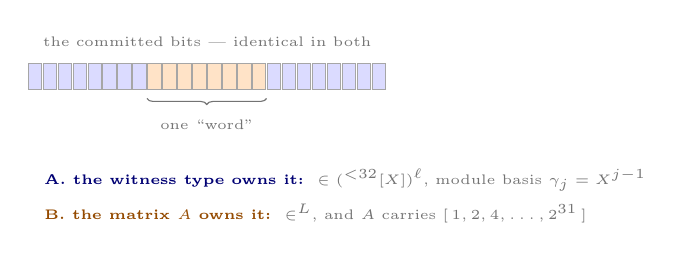
\begin{tikzpicture}[
  font=\scriptsize,
  bitc/.style={draw=black!35, minimum width=0.17cm, minimum height=0.34cm,
              inner sep=0pt, line width=0.25pt},
  hlA/.style={fill=blue!14}, hlB/.style={fill=orange!22},
  dcap/.style={font=\tiny, text=black!55, align=center},
  lbl/.style={font=\scriptsize\bfseries},
]
\foreach \k in {0,...,23} {
  \pgfmathsetmacro\bx{\k*0.19}
  \ifnum\k<8 \node[bitc, hlA] at (\bx,0) {}; \else
    \ifnum\k<16 \node[bitc, hlB] at (\bx,0) {}; \else
      \node[bitc, hlA] at (\bx,0) {}; \fi\fi
}
\node[dcap] at (2.19,0.44) {the committed bits --- identical in both};
\draw[decorate, decoration={brace, amplitude=2.2pt, mirror}, draw=black!55]
  (8*0.19-0.095,-0.28) -- (15*0.19+0.095,-0.28);
\node[dcap] at (2.19,-0.62) {one ``word''};

%% A and B stacked BELOW the strip: placed beside it they overlapped its right end.
\node[dcap, anchor=west, align=left] at (0,-1.32)
  {\textbf{\textcolor{blue!45!black}{A. the witness type owns it:}}\ \
   $\ff\in(\bits^{<32}[X])^{\ell}$, module basis $\gamma_j=X^{j-1}$};
\node[dcap, anchor=west, align=left] at (0,-1.74)
  {\textbf{\textcolor{orange!58!black}{B. the matrix $A$ owns it:}}\ \
   $\ff\in\bits^{L}$, and $A$ carries $[\,1,2,4,\dots,2^{31}\,]$};
\end{tikzpicture}
\end{center}

\begin{center}\small
\begin{tabular}{@{}p{0.14\textwidth}p{0.22\textwidth}p{0.23\textwidth}@{}}
\toprule
& \textbf{A. polynomial witness} & \textbf{B. bit witness}\\
\midrule
witness type & $(\Z^{\leq31}_{\leq B}[X])^{\ell}$ & $\bits^{L}$\\
$(d,B)$ & $d=31$, $B$ per column & $d=0$, $B=1$\\
grouping lives in & the module basis & $A$'s coefficients\\
$M$ outputs & words & bits\\
rotations, shifts & need $M$ --- a word-level $\ROTR$ is not $\Z$-linear
  & \textbf{free} --- a permuted coefficient pattern\\
modular addition & ideal $(X-2)$, carry monomial $X^{32}$ & plain $\Z$ row,
  carry term $2^{32}\mu$\\
ideals & required & none\\
opening carries & $\psi_M(\gamma_j)=\alpha^{j-1}$ in the coefficient vector
  & nothing extra\\
typing risk & shared $(d,B)$ pads $3$-bit carries to $32$ & none --- every cell
  is one bit\\
\bottomrule
\end{tabular}
\end{center}

The row that decides it for hashes is the fourth. Under A a rotation of a
\emph{word} is not a $\Z$-linear function of that word, so $M$ must manufacture
it and the result occupies a slot in $\hh$. Under B the word is already
$\sum_i b_i2^i$, so the rotation is the same coefficient pattern permuted --- and
costs nothing anywhere. That is what leaves $M$ responsible for XOR alone.

\paragraph{When the polynomial witness is the right choice.}
A is not a worse design; it is a design for a different workload. Where the
computation is \emph{natively} over a polynomial ring --- lattice signatures such
as Falcon, or anything in $R[X]/I$ --- the ideal earns its place, for the reason
in \cref{rem:noideals}: a product can be constrained as $c-ab\in I$ without
pinning down which representative of $c \bmod I$ the prover used. There is a
protocol-level argument too: ideal membership with the zero ideal degenerates to
univariate skip, so the general form is a \emph{generalised} univariate skip
rather than mere notation.

Hashes are the opposite case, and the reason is the next round: a register value
is immediately consumed bit-by-bit, so it must already be a minimal
representative and $c-ab\in I$ does not discharge the obligation.

\begin{remark}[One relation, two instantiations]\label{rem:oneinstance}
A and B are not competing systems. B is the degenerate case of the same
\textsc{PIMSAT} relation at $d=0$, $B=1$: the module collapses to $\Z$, $[X]$
goes unused, and the ideal becomes $(0)$. Nothing below the arithmetization
changes --- the commitment path of \cref{sec:commit}, the exponent fold, GKR, the
ring-switch and the proximity test are identical. Only the top layer differs.
\end{remark}

\subsection{All of SHA-256, in one table}\label{sec:shaspec}

SHA-256's compression function keeps eight $32$-bit registers $a,\dots,h$, runs
$64$ rounds, and first expands a $16$-word message block into a $64$-word
schedule. That is the whole of it --- and the whole of it fits in
\cref{tab:sha}.

Read the table with one convention: \textbf{every quantity is a $32$-bit word},
$+$ means addition modulo $2^{32}$, and $\xo$, $\wedge$, $\neg$ are bitwise XOR,
AND and NOT. $\ROTR^r$ rotates right by $r$; $\SHR^r$ shifts right by $r$ and
fills with zeros. Nothing else is needed.

\begin{center}\small
\begin{tabular}{@{}>{\raggedright\arraybackslash}p{0.13\textwidth}
                  >{\raggedright\arraybackslash}p{0.34\textwidth}
                  >{\raggedright\arraybackslash}p{0.21\textwidth}@{}}
\toprule
quantity & definition & where it goes\\
\midrule
\multicolumn{3}{@{}l}{\emph{Bit-mixing functions}}\\
$\Sigma_0(x)$ & $\ROTR^{2}(x)\xo\ROTR^{13}(x)\xo\ROTR^{22}(x)$
  & rotations free in $A$; XOR in $M$\\
$\Sigma_1(x)$ & $\ROTR^{6}(x)\xo\ROTR^{11}(x)\xo\ROTR^{25}(x)$ & same\\
$\sigma_0(x)$ & $\ROTR^{7}(x)\xo\ROTR^{18}(x)\xo\SHR^{3}(x)$ & same\\
$\sigma_1(x)$ & $\ROTR^{17}(x)\xo\ROTR^{19}(x)\xo\SHR^{10}(x)$ & same\\
$\Ch(x,y,z)$  & $(x\wedge y)\xo(\neg x\wedge z)$
  & $A$, via $2(a\wedge b)=a{+}b{-}(a\xo b)$\\
$\Maj(x,y,z)$ & $(x\wedge y)\xo(x\wedge z)\xo(y\wedge z)$ & same\\
\midrule
\multicolumn{3}{@{}l}{\emph{Message schedule}, $W_1\dots W_{64}$}\\
$W_t,\ t\leq16$ & $M_t$ \ \ (the input block) & $A$ --- a copy\\
$W_t,\ t>16$ & $W_{t-16}+\sigma_0(W_{t-15})+W_{t-7}+\sigma_1(W_{t-2})$
  & $A$ --- one addition row\\
\midrule
\multicolumn{3}{@{}l}{\emph{Round $t$}, on state $(a,\dots,h)$}\\
$T_1$ & $h+\Sigma_1(e)+\Ch(e,f,g)+K_t+W_t$ & $A$\\
$T_2$ & $\Sigma_0(a)+\Maj(a,b,c)$ & $A$\\
$a_{t+1}$ & $T_1+T_2$ & $A$\\
$e_{t+1}$ & $d+T_1$ & $A$\\
the rest & $(b,c,d,f,g,h)_{t+1}=(a,b,c,e,f,g)_t$
  & \textbf{free} --- a shift register\\
\midrule
\multicolumn{3}{@{}l}{\emph{Output}, after $64$ rounds}\\
$H^{\mathrm{out}}_j$ & $S^{\mathrm{in}}_j+S^{\mathrm{fin}}_j$, $j\in\{0,\dots,7\}$
  & $A$ --- eight addition rows\\
\bottomrule
\end{tabular}
\captionof{table}{SHA-256 in full. All values are $32$-bit words; $+$ is modulo
$2^{32}$. The right column is this document's thesis in miniature.}
\label{tab:sha}
\end{center}

\paragraph{Reading the right-hand column.}
Fourteen lines, and only two kinds of work in them.

\begin{itemize}[leftmargin=1.4em,itemsep=2pt,topsep=4pt]
  \item \textbf{Six lines shuffle bits} --- the $\Sigma$s, $\sigma$s, $\Ch$ and
        $\Maj$. Their rotations and shifts are free (permuted power-of-two
        diagonals in $A$), their XORs go to $M$, and their $\wedge$s are the only
        genuinely nonlinear thing in SHA-256.
  \item \textbf{Seven lines add} --- schedule, $T_1$, $T_2$, the two register
        updates, and the output. Each is one row of $A$ with one small carry.
  \item \textbf{One line is free.} The shift register is why only $a$ and $e$
        need committed columns: $b_t=a_{t-1}$, $c_t=a_{t-2}$, $d_t=a_{t-3}$, and
        likewise $f,g,h$ off $e$.
\end{itemize}

\noindent
So the $\wedge$s are the whole difficulty, there are only two of them per round
in $\Ch$ and three in $\Maj$, and \cref{sec:Amatrix} disposes of both with a
single identity.

\subsection{Public parameters, committed bits, and the virtual witness}

\begin{center}\small
\begin{tabular}{@{}llll@{}}
\toprule
& contents & bits / compression & committed?\\
\midrule
$\xx$ & IV, digest, message block, the $K_t$ & --- & public\\
$\ff$ & $a,e,W$ bit columns $+$ carries $\mu_a,\mu_e,\mu_W$
  & $\approx6\,800$ & \textbf{yes}\\
$\hh$ & $\ff$ \emph{stacked with} $\Sigma_0,\Sigma_1,\sigma_0,\sigma_1$,
  $X_{ef},X_{eg},X_{\mathrm{maj}}$ & $\approx20\,100$ & \textbf{no}\\
\bottomrule
\end{tabular}
\end{center}

Everything in the two witness vectors is a bit.  The public input $\xx$
parameterizes the matrix $A_{\xx}$; it is not a third PIOP witness block.
There is no module, no degree bound and no $(d,B)$ pair;
$\bitsop(\ff)=\ff$.

\begin{warning}[$\hh$ includes $\ff$, and the grand product runs over all of it]
\label{warn:hsize}
$M$ is taken in stacked form, with a verifier-known constant row and
$[\,\mathrm{Id}\,;\,M_{\rm xor}\,]$ on the committed tail, so
$\hh=(1,\ff,\text{derived})$ --- the paper's own example defines
$M\cdot\pitwo(\ff)$ as the \emph{concatenation} of $\pitwo(\ff)$ with the
derived vector. The grand product therefore folds
$\approx20\,100$ bits per compression, not the $\approx13\,300$ of the derived
block alone. Costing the forest against the narrower figure undercounts it by
about a third. Both numbers here are \textbf{derived}, not measured --- no
SHA-256 witness generator exists in the repository yet.
\end{warning}

The registers $b,c,d,f,g,h$ need no columns --- SHA-256's state update is a shift
register, so $b_t=a[t{-}1]$, $c_t=a[t{-}2]$, $d_t=a[t{-}3]$ and likewise
$f,g,h$ off $e$. Only $a$ and $e$ are stored. Both the initial \emph{and} final
states are public input, so the trace is $64$ rows, not $65$, which keeps the
row axis at $2^6$ instead of padding to $2^7$.

\subsection{$M$: the XOR matrix}

$M\in\Ftwo^{|\hh|\times|\ff^{\circ}|}$, where
$\ff^{\circ}=(1,\ff)$, is a bit matrix and part of the \emph{public}
input. Each output bit is the XOR of a few committed bits:

\begin{center}\small
\begin{tabular}{@{}lll@{}}
\toprule
family & output bit $i$ & ones/row\\
\midrule
$\Sigma_0[t]$ & $a[t]_{i+2}\xo a[t]_{i+13}\xo a[t]_{i+22}$, indices mod $32$ & 3\\
$\Sigma_1[t]$ & $e[t]_{i+6}\xo e[t]_{i+11}\xo e[t]_{i+25}$ & 3\\
$\sigma_0[s]$ & $W[s]_{i+7}\xo W[s]_{i+18}\xo W[s]_{i+3}$, last term iff $i\leq28$ & 3 / 2\\
$\sigma_1[s]$ & $W[s]_{i+17}\xo W[s]_{i+19}\xo W[s]_{i+10}$, last term iff $i\leq21$ & 3 / 2\\
$X_{ef}[t]$ & $e[t]_i \xo e[t{-}1]_i$ & 2\\
$X_{eg}[t]$ & $e[t]_i \xo e[t{-}2]_i$ & 2\\
$X_{\mathrm{maj}}[t]$ & $a[t]_i \xo a[t{-}1]_i \xo a[t{-}2]_i$ & 3\\
\bottomrule
\end{tabular}
\end{center}

The rotation amounts appear as \emph{index offsets}, not as rotation
operations --- because $M$ indexes bits directly, a rotated read is simply a
different column. $\SHR$ is truncated rather than cyclic, so the $\sigma$ rows
near the top carry one fewer entry; treating those blocks as circulant is a
silent correctness bug.

\begin{warning}[Bit rotations are free; \emph{word offsets} are not]
\label{warn:offsets}
It is tempting to say ``all of $\hh$ is re-indexing, therefore all of $\hh$ is
free.'' That is true for four of the seven families and false for three.

A bit rotation stays inside the clear axis, and a tap body is $2^{t'+s_x}$
leaves whatever the taps are --- \textbf{measured}, seven tap shapes at $n{=}22$
all land in a $\pm10\%$ band with no ordering by shape. A \emph{word offset},
though, carries out of the clear axis and breaks the row\,$\otimes$\,column
tensor, which \textbf{doubles the inner body count}: measured at $n{=}22$ with
identical claim counts, eight pure-offset claims cost $85.9$\,ms against
$56.1$\,ms for eight pure rotations --- $+55\%$ prove, $+60\%$ verify, $+39\%$
bytes.

$\Sigma_0,\Sigma_1,\sigma_0,\sigma_1$ read one column at rotated positions and
are free. $X_{ef},X_{eg},X_{\mathrm{maj}}$ read \emph{adjacent rows}
($a[t{-}1]$, $e[t{-}2]$, \dots) and are pure word offsets. If a cheaper
arithmetization exists, that is where to look.
\end{warning}

\paragraph{What $M$ hands to $A$.} $M$ produces \emph{bits} --- one per row,
each the XOR of two or three committed bits, $13\,312$ of them per compression
(\cref{sec:census}). The lift $\pitwo^{-1}$ puts them back in
$\bits\subseteq\Z$, the same type $\ff$ already has.  After adding the
constant coordinate and substituting the public data into the coefficients,
\[
  \hh=\pitwo^{-1}\!\bigl(M\pitwo(\ff^{\circ})\bigr)\in\bits^n,
  \qquad A_{\xx}\hh=0.
\]
So the PIOP sees one flat bit vector.  An $\hh$
column is a bit column, indexed and weighted exactly like a committed-bit
identity row. A
term such as $\Sigma_0[t]$ enters a row of $A$ as $2^0,\dots,2^{31}$ on the $32$
bits of that family, precisely as $e[t{-}3]$ does on committed bits. The only
difference between the two blocks is that one is behind the Merkle root and the
other is not --- which is a statement about \cref{sec:commit}, not about $A$.

That seam is what the whole construction turns on. $M$ is linear over $\Ftwo$,
where XOR is free and carries are meaningless; $A_{\xx}$ is linear over $\Z$, where
carries are the point and XOR is unavailable. They compose because \emph{they
index the same bits}: the only object crossing between them is the bit vector
itself. What is \emph{not} linear is the lift $\pitwo^{-1}$ sitting between the
two --- and \cref{step:transpose} is where that bill comes due, at Step~8.

\subsection{$A$: the \texorpdfstring{$\Z$}{Z}-linear system}\label{sec:Amatrix}

$\Ch$ and $\Maj$ are the only nonlinear gates, and both become linear once the
XOR is available in $\hh$. Per bit $x\andop y=(x+y-(x\xo y))/2$; and since
$e\andop f$ and $\notop e\andop g$ have disjoint bit support their XOR is their
integer sum, with the complement's constants cancelling:
\begin{align}
  2\,\Ch[t]  &= e[t{-}1] + e[t{-}2] - X_{ef}[t] + X_{eg}[t], \label{eq:ch}\\
  2\,\Maj[t] &= a[t] + a[t{-}1] + a[t{-}2] - X_{\mathrm{maj}}[t]. \label{eq:maj}
\end{align}
Both hold coefficient-wise --- every coefficient of the right-hand side is $0$ or
$2$ --- so the halving involves no carry propagation. Neither is a row of $A$;
both fold into the update rows below.

\paragraph{The three interior templates.} Written as they read, these are
exactly the round and schedule lines of \cref{tab:sha} with the shift-register
substitutions $h_t=e[t{-}3]$ and $d_t=a[t{-}3]$ made, and the modular reduction
turned into an explicit carry:

\begin{center}\small
\begin{tabular}{@{}llc@{}}
\toprule
& constraint over $\Z$ & rows $t$\\
\midrule
$C_1$ & $a[t{+}1] = e[t{-}3] + \Sigma_1[t] + \Ch[t] + \mathbf y_K[t] + W[t]
        + \Sigma_0[t] + \Maj[t] - 2^{32}\mu_a[t]$ & $[1..64]$\\[3pt]
$C_2$ & $e[t{+}1] = a[t{-}3] + e[t{-}3] + \Sigma_1[t] + \Ch[t]
        + \mathbf y_K[t] + W[t] - 2^{32}\mu_e[t]$ & $[1..64]$\\[3pt]
$C_3$ & $W[t] = W[t{-}16] + \sigma_0[t{-}15] + W[t{-}7] + \sigma_1[t{-}2]
        - 2^{32}\mu_W[t]$ & $[17..64]$\\
\bottomrule
\end{tabular}
\end{center}

Every symbol denotes a \emph{word}, and every word is itself a row of
power-of-two coefficients over the underlying bits. Expanded, a term like
$\Sigma_0[t]$ contributes coefficients $2^0,\dots,2^{31}$ on the $32$ bits of
that $\hh$ family, and $e[t{-}3]$ contributes the same on committed bits.
Rotations --- had they not already been absorbed into $M$ --- would appear here as
a \emph{permutation} of those coefficients, which is the content of move (ii).

\begin{remark}[Where the halves go]\label{rem:doubling}
$\Ch[t]$ and $\Maj[t]$ above are the \emph{halves} of \eqref{eq:ch} and
\eqref{eq:maj}, so substituting them into $C_1$ and $C_2$ introduces
coefficients of $\tfrac12$. The stored rows are therefore doubled --- which is
free, since $2p=0 \iff p=0$ over $\Z$ --- turning every $\tfrac12$ into $1$,
every $1$ into $2$, and the carry term $2^{32}\mu$ into $2^{33}\mu$. That is a
bookkeeping step, not a modelling one, and it is why \textbf{no $2^{-1}$ ever
appears}: over $\Fq$ the coefficient $\pm(q{+}1)/2$ would be a full-width field
element on nine of $C_1$'s entries.
\end{remark}

\paragraph{The boundary rows.} Thirty of them, in four groups.

\begin{center}\small
\begin{tabular}{@{}lcl@{}}
\toprule
group & rows & equations\\
\midrule
prologue & $6$ & $a[0]=\mathbf y_b[1]$,\ \ $a[{-}1]=\mathbf y_c[1]$,\ \
  $a[{-}2]=\mathbf y_d[1]$\\
 & & $e[0]=\mathbf y_f[1]$,\ \ $e[{-}1]=\mathbf y_g[1]$,\ \
  $e[{-}2]=\mathbf y_h[1]$\\[3pt]
initial state & $2$ & $a[1]=\mathbf y_a[1]$,\ \ $e[1]=\mathbf y_e[1]$\\[3pt]
schedule init & $16$ & $W[t]=\mathbf y_M[t]$,\ \ $t\in[1..16]$\\[3pt]
final state & $6$ & $a[64]=\mathbf y_b[65]$,\ \ $a[63]=\mathbf y_c[65]$,\ \
  $a[62]=\mathbf y_d[65]$\\
 & & $e[64]=\mathbf y_f[65]$,\ \ $e[63]=\mathbf y_g[65]$,\ \
  $e[62]=\mathbf y_h[65]$\\
\midrule
 & $\mathbf{30}$ & all with ideal $(0)$ --- plain equalities, no carry\\
\bottomrule
\end{tabular}
\end{center}

Three of these groups need a word of explanation.

\begin{itemize}[leftmargin=1.4em,itemsep=3pt,topsep=4pt]
  \item \textbf{The prologue exists so that $C_1$--$C_3$ are uniform.} The shift
        register reads $b_t=a[t{-}1]$, $c_t=a[t{-}2]$, $d_t=a[t{-}3]$, so at
        $t\leq3$ those references fall before row $1$. Committing three extra
        cells on each of $a$ and $e$ --- holding the public IV words
        $b_1,c_1,d_1$ and $f_1,g_1,h_1$ --- makes the window total on $[1..64]$
        and \textbf{eliminates every special-case row}. Six cells, and Table 8
        and Table 9 of Zinc\raisebox{0.1ex}{+} both disappear.
  \item \textbf{The final state is pinned at rows $62$--$64$}, not $65$, for the
        same reason read forwards: $b_{65}=a_{64}$, $c_{65}=a_{63}$,
        $d_{65}=a_{62}$.
  \item \textbf{$a[65]$ and $e[65]$ get no rows at all.} They are public, so
        $\mathbf y_a[65]$ and $\mathbf y_e[65]$ are substituted directly for the
        left-hand sides of $C_1$ and $C_2$ at $t=64$. That keeps the trace at
        $64$ rows rather than padding the row axis from $2^6$ to $2^7$.
\end{itemize}

\paragraph{Every entry of $A$.}
$\{0\}\cup\{\pm2^j : 0\leq j\leq 35\}$, and nothing else. Trace the exponents
through \cref{rem:doubling} rather than reading them off the undoubled rows,
because the doubling moves every one of them:
\begin{itemize}[leftmargin=1.4em,itemsep=2pt,topsep=4pt]
  \item $C_1,C_2$ are \emph{doubled}, so word assembly occupies
        $2^1,\dots,2^{32}$ and the carry term is $2^{33}\mu$. Since $\mu_a,\mu_e$
        are three \emph{bit} columns of weights $1,2,4$, the carry entries are
        $2^{33},2^{34},2^{35}$ --- so $\mathbf{j=35}$, on the top carry bit.
  \item $C_3$ carries no half, so it is \emph{not} doubled: word assembly
        $2^0,\dots,2^{31}$, and the $2$-bit $\mu_W$ at weight $2^{32}$ gives
        $2^{32},2^{33}$. So $j\leq33$ there.
  \item Boundary rows are \emph{word} equations --- six prologue rows, not
        $6\times32$ --- so each carries the full assembly diagonal
        $\pm2^0,\dots,\pm2^{31}$ on the committed side, with the public word on
        the $\xx$ side. \textbf{They are not $\pm1$ rows.}
\end{itemize}
Nothing downstream moves: $2^{35}$ is still far below $q\approx2^{100}$, and the
residual bound of \cref{step:project} is unchanged.

\subsection{What this removes}

\begin{center}\small
\begin{tabular}{@{}p{0.26\textwidth}lp{0.24\textwidth}@{}}
\toprule
Zinc\raisebox{0.1ex}{+} item & status & why\\
\midrule
$\Sigma,\sigma$ in $\Ftwo[X]/(X^{32}{-}1)$ & \textbf{gone} & absorbed into $M$\\
the $\Ftwo[X]$ trace component & \textbf{gone} & those rows were its only content\\
$\Ch$/$\Maj$ lookups & \textbf{gone} & \eqref{eq:ch}, \eqref{eq:maj}\\
columns $\Maj,u_{ef},u_{\neg e,g}$ & \textbf{gone} & inline expressions\\
ten bit-ness lookups & \textbf{gone} & F2Z commits the bits\\
range lookups on $\mu$ & \textbf{gone} & a 3-bit cell \emph{is} $\rge{0}{7}$\\
\textbf{the ideals} $(X{-}2)$, $(X^{32}{-}1)$ & \textbf{gone} & \cref{rem:noideals}\\
the module $\Z^{\leq d}_{\leq B}[X]$, $\bitsop(\cdot)$ & \textbf{gone} & the witness is already bits\\
\bottomrule
\end{tabular}
\end{center}

\begin{warning}[Bit-ness is a precondition --- and \cref{step:proximity} is what
discharges it]\label{warn:bitness}
Deleting the bit-ness lookups is sound \emph{only} if every cell of $\ff$ really
lies in $\bits$, and the identity $2(a\andop b)=a+b-(a\xo b)$ leans on the same
guarantee, so it is load-bearing in two places. It is worth being precise about
where it comes from, because the answer is not ``a constraint''.

\textbf{Nothing enforces bit-ness. The message space has no non-bits in it.}
The code $\cC$ has dimension $N/128$ over $\comfield$, so an accepted codeword's
message lives in $\comfield^{N/128}$; and $\pack$ is an $\Ftwo$-linear
\emph{bijection} $\Ftwo^{N}\to\comfield^{N/128}$, being a change of basis on an
$\Ftwo$-space of dimension $N$. Unpacking any accepted message therefore yields
a vector over $\Ftwo$, and lifting gives $\bits\subseteq\Z$. A prover cannot
place a $2$ in a bit slot, because the slot is one \emph{bit of a field element},
not an integer cell.

Read it in extractor terms and it is one line: the proximity test's extractor
returns $\comfield$ elements; undoing the packing and the projection returns
integer bits; there is no branch in which it returns anything else. Equivalently,
every value the protocol actually \emph{reads} is a bit --- the exponent fold of
\cref{step:exponent} consumes $\pitwo(H[\rowidx,\colidx])$, never a raw integer --- so
a claimed witness carrying a $2$ is simply not a witness the relation
recognises.

\textbf{The caveat.} This is a statement about the \emph{extracted} witness, so
it holds up to the proximity error and the list-decoding radius of $\cC_1$ ---
exactly like the binding claim $C$ it travels with (\cref{step:proximity}). It
is not an unconditional typing guarantee; it is precisely as sound as the
opening, which is the right place for it to live.

\textbf{And this argument is ours, not the paper's --- but the surrounding
theorem is not missing.} Earlier drafts of this note said the core-IOP soundness
theorem was an empty stub whose proof stopped at \code{WIP}. \textbf{That was
read off a stale checkout and is false.} In the current source the core-IOP
theorem is stated with explicit hypotheses --- including
$\ord(\gen)>(\ellrow{+}1)(q_{\max}{-}1)$ --- and its proof runs to a full
\code{\textbackslash end\{proof\}}, decomposing the construction, exhibiting the
knowledge-state function and the round-by-round extractor, and proving its own
reduction lemma. The only thing flagged missing on it is
\emph{completeness}; the only \code{WIP} markers anywhere in the paper are in the
introduction's benchmark prose. Of the three theorems, exactly one --- the
\emph{virtualized} variant --- is still an empty statement--proof pair, and that
is the one this note actually depends on.

So the accurate claim is narrower and more useful: the composition framework and
the core theorem are both there; what is missing is the theorem for the
virtualized relation, and the bit-ness argument above is a natural extractor
construction filling a gap the paper leaves at \emph{that} level rather than at
the base.

The paper does name the gap, and it is worth reading precisely. Construction
5.3's proof sketch says the F2Z IOP \emph{``has already been studied, except that
we started with $\ff$ containing only bits, so we need to add a wrapper around
it''}, marked \code{todo}. That wrapper is needed for a \textbf{module} witness,
not for a bit one: with entries in $R^{\leq d}_{\leq B}[X]$ the extractor yields
bits, and something must then reassemble module elements from them and re-check
the bounds $(d,B)$. With a bit witness there is nothing to reassemble and no
bound to re-verify --- the witness \emph{is} the extracted object. The design of
this note therefore sidesteps the one soundness gap the paper leaves explicitly
open, which is a better argument for \cref{sec:typing}'s choice than any of the
ones given there.
\end{warning}

\begin{remark}[The typing problem, and why it is gone]\label{rem:typing}
With a polynomial witness, word cells want $(d,B)=(32,1)$ while carry cells want
$(1,3)$, and the relation fixes \emph{one} global pair --- so everything pads to
the maximum and the committed size becomes $\ell\cdot32\cdot32$ where
$\ell\cdot32$ would do. On the paper's own figures that padding lands on exactly
$2^{14}$ bits per compression: the unvirtualized baseline, i.e.\ \emph{zero}
gain from virtualization. Zinc\raisebox{0.1ex}{+} does not escape it either --- its
degree bound is indexed per trace component, not per column.

With a bit witness the question does not arise. $D=B=1$, there is nothing to
pad, and $|\ff|\approx6\,800$ bits stands. This is the strongest single argument
for dropping the ideals, and it is not the one usually given.
\end{remark}

\subsection{The complete census}\label{sec:census}

Everything in this section, counted. One compression --- one $512$-bit block ---
and the whole system is two blocks that are not commensurable, which is the
point.

\paragraph{$M$: the virtual XOR rows, over $\Ftwo$.} One row per \emph{output
bit}. $M$ is public, so none of this is committed and none of it is proved
directly.

\begin{center}\small
\begin{tabular}{@{}llrrcr@{}}
\toprule
family & instances & words & rows & ones/row & nonzeros\\
\midrule
$\Sigma_0[t]$          & $t\in[1..64]$   & $64$ & $2\,048$ & $3$     & $6\,144$\\
$\Sigma_1[t]$          & $t\in[1..64]$   & $64$ & $2\,048$ & $3$     & $6\,144$\\
$\sigma_0[s]$          & $s\in[2..49]$   & $48$ & $1\,536$ & $3$ / $2$ & $4\,464$\\
$\sigma_1[s]$          & $s\in[15..62]$  & $48$ & $1\,536$ & $3$ / $2$ & $4\,128$\\
$X_{ef}[t]$            & $t\in[1..64]$   & $64$ & $2\,048$ & $2$     & $4\,096$\\
$X_{eg}[t]$            & $t\in[1..64]$   & $64$ & $2\,048$ & $2$     & $4\,096$\\
$X_{\mathrm{maj}}[t]$  & $t\in[1..64]$   & $64$ & $2\,048$ & $3$     & $6\,144$\\
\midrule
\textbf{total}         &                 & $\mathbf{416}$ & $\mathbf{13\,312}$
                       &                 & $\mathbf{35\,216}$\\
\bottomrule
\end{tabular}
\end{center}

\noindent
The $\sigma$ rows are the only ragged ones: $\SHR^3$ and $\SHR^{10}$ truncate, so
$3$ and $10$ of their output bits respectively carry two entries instead of
three. Stacked as $M'=[\,\mathrm{Id};M\,]$ (\cref{warn:hsize}) the derived
$13\,312$ bits join $\ff$'s $6\,816$ to give $|\hh|=20\,128$.

\paragraph{$A$: the constraint rows, over $\Z$.} One row per \emph{word
equation}. These are the constraints in the PIOP sense --- the rows the
zero-check of \cref{sec:piop} runs over.

\begin{center}\small
\begin{tabular}{@{}llrll@{}}
\toprule
family & rows $t$ & rows & carry & entries\\
\midrule
$C_1$ \ $a$-update      & $[1..64]$  & $64$  & $\mu_a$, $3$ bits & $\pm2^j$, $1\leq j\leq35$\\
$C_2$ \ $e$-update      & $[1..64]$  & $64$  & $\mu_e$, $3$ bits & $\pm2^j$, $1\leq j\leq35$\\
$C_3$ \ schedule        & $[17..64]$ & $48$  & $\mu_W$, $2$ bits & $\pm2^j$, $j\leq33$\\
\midrule
prologue                & ---        & $6$   & --- & $\pm2^j$, $j\leq31$\\
initial state           & ---        & $2$   & --- & $\pm2^j$, $j\leq31$\\
schedule init           & $[1..16]$  & $16$  & --- & $\pm2^j$, $j\leq31$\\
final state             & ---        & $6$   & --- & $\pm2^j$, $j\leq31$\\
\midrule
\textbf{total}          &            & $\mathbf{206}$ & & \\
\bottomrule
\end{tabular}
\end{center}

\noindent
\begin{remark}[Why $206$ looks impossibly small]\label{rem:rowsvswidth}
It is a \emph{row} count, and the rows are wide. One row of $A$ absorbs an
entire $32$-bit modular addition, because over $\Z$ the carry propagation is
carried by the equation's \emph{value} rather than by extra constraints ---
which is what the $\pm2^j$ coefficients buy. Count a $C_1$ row honestly, with
$\Ch$ and $\Maj$ \emph{expanded} --- neither is a column, and between them they
contribute eight word blocks:
\begin{align*}
  &\underbrace{a[t{+}1],\,e[t{-}3],\,\Sigma_1,\,W,\,\Sigma_0}_{5}
  \;+\;\underbrace{e[t{-}1],e[t{-}2],X_{ef},X_{eg}}_{\Ch,\ 4}\\[-2pt]
  &\qquad
  +\underbrace{a[t],a[t{-}1],a[t{-}2],X_{\mathrm{maj}}}_{\Maj,\ 4}
  \;+\;\underbrace{\mathbf y_K}_{\text{public}}
\end{align*}
--- $14$ word blocks, matching \cref{step:project}'s ``$\leq15$ word terms''.
That is $14\times32+3=\mathbf{451}$ nonzero bit columns, not $300$.

Multiply through and the two counts reconcile:
$64(451)+64(323)+48(162)+30(64)=\mathbf{59\,232}$ bit-level nonzeros --- the
$\mathrm{nnz}_{\mathrm{bit}}(\bar A_0)$ that \cref{step:collapse} charges the
verifier for. \textbf{Nothing was saved; it moved from row count to row width.}

The saving that \emph{is} real shows up against characteristic $2$. There a
$32$-bit modular addition needs a ripple-carry circuit --- on the order of $32$
rows plus $32$ fresh AND variables per addition. Across the $176$ word additions
here ($64+64+48$) that is $\sim\!5\,600$ rows and $\sim\!5\,600$ carry
variables, against $176$ rows and $\sim\!500$ carry \emph{bits} over $\Z$:
roughly $30\times$ fewer constraints, and the reason the ring is $\Z$ at all.
These are derived counts, not measured.
\end{remark}

\noindent
\textbf{The rows are word equations; the columns are bits.} Nothing in $\hh$ is
a $32$-bit integer --- every variable is in $\bits$, carries included, and a
word never exists as a stored quantity. A row of $A$ \emph{assembles} it:
$\sum_{j=0}^{31}2^j b_j$, which is what the assembly entries are for. In the
doubled rows that band is $2^1,\dots,2^{32}$, and the carry sits above it at
$2^{33}\!\cdot\!\{1,2,4\}=2^{33},2^{34},2^{35}$ --- so even $\mu_a$ is three
\emph{bit columns}, not a small integer, and it is the doubling that puts the
top one at $2^{35}$. Integers appear only as \emph{values}: the
residual $\ipZ{A[\beta,*]}{\hh}$ reaches $\approx2^{37}$, comfortably inside the
$\approx2^{40}$ bound \cref{step:project} argues for. \textbf{Integers are values here, never
variables} --- and reading the table the other way is what produces the
word-versus-bit granularity slips flagged in \cref{step:collapse}.

Index a constraint by (family, round): four families $\times$ $64$ rounds is
$2^8$ slots, of which $206$ are live --- an $80.5\%$ fill, and $\nu=8$ for the
zero-check. The $50$ dead slots are $C_3$'s first sixteen rounds and the
boundary block's remainder; padding them with the zero row is free. This is the $64$-round
loop alone; the feed-forward addition (open item~7, \cref{sec:config}) would add
eight more rows and eight one-bit carries, taking $A$ to $214$.

\paragraph{The total, and why the two halves must be counted separately.}

\begin{center}\small
\begin{tabular}{@{}llrl@{}}
\toprule
& ring & rows & discharged by\\
\midrule
$M$ & $\Ftwo$ & $13\,312$ & one transposition, \cref{step:transpose}\\
$A$ & $\Z$    & $206$     & the zero-check, \cref{sec:piop}\\
\midrule
\textbf{total} & & $\mathbf{13\,518}$ & \\
\bottomrule
\end{tabular}
\end{center}

\noindent
Adding those two numbers is almost meaningless, and the reason is the whole
design. $A$'s $206$ rows are constraints in the ordinary sense: the prover is
proving them, and they set the size of the public vector $\vv_0$ the verifier builds in
\cref{step:collapse}. They are \emph{not} the dimension of either
prover-wide pass.  The evaluation-shaping sumcheck of \cref{step:eqshape} scans
the padded $\hh$ table once, and the grand-product forest of \cref{step:gkr}
scans it again; both scale with $|\hh|$, not with the $206$ row count.
$M$'s $13\,312$ rows are \emph{definitions} --- they say what $\hh$ is, they are
public, and \cref{sec:iopp} discharges all of them at once by transposing a
single linear form. Neither the prover nor the verifier ever touches a row of
$M$ individually.

So the honest headline is: \textbf{$206$ constraints per compression}, plus a
public $13\,312$-row rewrite that costs one transpose. For $L$ blocks both
scale linearly --- $206L$ and $13\,312L$ --- with $\nu=8+\lceil\log_2 L\rceil$
and the committed witness at $6\,816L$ \emph{useful} bits --- which is not what
gets committed.

\begin{warning}[These are useful-bit counts. What is committed is a
rectangle]\label{warn:laidout}
Every figure above --- $|\ff|=6\,816$, $|\hh|=20\,128$, the per-family row
counts --- is a \emph{ragged} sum over roles. The object that is actually
committed, encoded and folded is a rectangular tensor whose size is set by three
independent power-of-two axes \src{\code{cells()} --- src/pcs.rs}:
\begin{center}
\small
\(
  \text{committed bits/compression}
  =
  2^{\,\log\mathrm{cols}+\mathtt{bit\_vars}+\mathtt{num\_vars}}
  =
  (\text{roles})\times32\times(\text{trace rows}),
\)
\end{center}
and \code{sha\_f2\_bit\_tensor} states the rule plainly: ``padding columns
($i\geq\code{num\_cols}$) and padding rows stay $0$''. Both of the non-trivial
axes are padded here:

\begin{center}\small
\begin{tabular}{@{}lrrrr@{}}
\toprule
& roles & rows & laid out & fill\\
\midrule
committed & $4$ & $128$ & $16\,384$ & $\mathbf{41.6\%}$\\
folded ($11$ virtual instances) & --- & --- & $45\,056$ & $\mathbf{44.7\%}$\\
\bottomrule
\end{tabular}
\end{center}

\noindent
The row axis is $128$, not $64$, because $\hat a$ and $\hat e$ span
$t\in[-2..64]=67$ cells and $67$ pads to $2^7$ --- which is the opposite of what
\S\ref{sec:arith} claims twice (``keeps the row axis at $2^6$ instead of padding
to $2^7$''). \textbf{That single sentence hides a factor of $1.91$ on the
largest object in the system.} Two consequences worth carrying:
\begin{itemize}[leftmargin=1.4em,itemsep=2pt,topsep=4pt]
  \item Every cost in \cref{sec:config} that is charged against $|\ff|$ or
        $|\hh|$ is charged against the wrong number, by $2.40\times$ and
        $2.24\times$ respectively.
  \item The two reducible levers are therefore \emph{padding}, not
        arithmetization: get the row axis to $64$ (substitute the public IV at
        $t=1,2,3$ exactly as $a[65],e[65]$ are already substituted at the top
        edge, which costs an affine $M$: $\hh=M\pitwo(\ff)\oplus\kappa$ with
        $\kappa$ public), and pin the role count at $4$. Each is worth exactly
        $2\times$; together they take the committed overhead from $2.40\times$
        to $1.24\times$.
\end{itemize}
\end{warning}

\begin{remark}[Is $6\,816$ a lot? Against four denominators]\label{rem:isitalot}
The width of $A$ --- $30\,016$ columns --- does not determine commitment or
oracle size: two thirds of it is $\hh$, which is never committed or sent, and a
tenth is public input.  It does, however, determine prover work through the
evaluation-shaping and grand-product passes over $\hh$.  (And $6\,816$ of it is
$\ff$ counted twice, since $\hh\supseteq\ff$.)  The number controlling the
committed oracle is $|\ff|=6\,816$ bits $=852$ bytes per compression.

\begin{center}\small
\begin{tabular}{@{}lrl@{}}
\toprule
against & ratio & \\
\midrule
the trace a prover must materialise anyway & $1.11\times$
  & $64\,a+64\,e+64\,W=6\,144$ bits\\
Zinc\raisebox{0.1ex}{+}, like-for-like content & $3.1\times$
  & $21\,385$ bits un-padded\\
Zinc\raisebox{0.1ex}{+} as typed, $(d,B)=(32,32)$ & $127\times$
  & flattered by padding --- see below\\
the raw block $+$ chaining state & $8.9\times$
  & $96$ bytes in, $852$ out\\
\bottomrule
\end{tabular}
\end{center}

\noindent
The first row is the real answer: \textbf{the committed witness is the trace
plus $11\%$}. The $672$-bit surcharge is six prologue words ($192$ bits, bought
to eliminate every special-case row) and $480$ carry bits. No auxiliary column,
no lookup table, no permutation argument, no bit-decomposition helper.

The last two rows deserve care. $127\times$ is arithmetically right and
misleading: it splits as $\sim\!3.1\times$ from virtualization and $\sim\!40\times$
from Zinc\raisebox{0.1ex}{+}'s \emph{shared} $(d,B)$ typing, which is
\cref{rem:typing}'s complaint rather than a property of this design. Restricted
to the columns both schemes commit, the two are a \textbf{dead heat} --- $6\,825$
against $6\,816$. F2Z found no tighter encoding of the trace; it moved seven
columns from committed to virtual and made thirteen lookups vacuous. That is the
honest claim.

Two caveats. $6\,816$ pads to $2^{13}$, an $83\%$ fill. And the whole census is
\textbf{derived, not measured} --- no SHA-256 witness generator exists in this
repository, so nothing here has ever been proved.
\end{remark}

\begin{remark}[What this replaces]
Zinc\raisebox{0.1ex}{+} spends ten constraint families over two rings on the same
computation, plus thirteen lookup arguments (ten for bit-ness, three for
$\Ch$/$\Maj$), on a $65\times13$ trace typed at $(d,B)=(32,32)$. The census above
is three interior families, one ring, no lookups, and the $\Ftwo$ half is not
proved at all. \cref{sec:config} carries the parameter-level comparison.
\end{remark}
